\newcommand{\NWtarget}[2]{#2}
\newcommand{\NWlink}[2]{#2}
\newcommand{\NWtxtMacroDefBy}{Fragment defined by}
\newcommand{\NWtxtMacroRefIn}{Fragment referenced in}
\newcommand{\NWtxtMacroNoRef}{Fragment never referenced}
\newcommand{\NWtxtDefBy}{Defined by}
\newcommand{\NWtxtRefIn}{Referenced in}
\newcommand{\NWtxtNoRef}{Not referenced}
\newcommand{\NWtxtFileDefBy}{File defined by}
\newcommand{\NWtxtIdentDefinedIn}{defined in}
\newcommand{\NWtxtIdentUsedIn}{used in}
\newcommand{\NWtxtIdentUsers}{Users:}
\newcommand{\NWtxtIdentsNotUsed}{never used}
\newcommand{\NWtxtIdentsUsed}{Uses:}
\newcommand{\NWsep}{${\diamond}$}
\newcommand{\NWnotglobal}{(not defined globally)}
\newcommand{\NWuseHyperlinks}{}
\documentclass[a4paper, 12pt]{article}
\usepackage{fullpage} % for 1.5 cm margins
\renewcommand{\familydefault}{\sfdefault} % so it doesn't look like LaTeX
\usepackage{helvet}
\usepackage{graphicx}
\graphicspath{ {imgs/} }
\usepackage{float} % so the figures stay with the text

\usepackage{abstract}
\renewcommand{\abstractname}{Overview}
\raggedright

\usepackage{parskip}

\usepackage{hyperref}
\hypersetup{
    colorlinks=true,
    linkcolor=blue,
    filecolor=magenta,      
    urlcolor=cyan,
}

\title{Promethean Temperature Sensor}
\author{Joe Collins}

\begin{document}
\maketitle
%%%%%%%%%%%%%%%%%%%%%%%%%%%%%%%%%%%%%%%%%%%%%%%%%%%%%%%%%%%%
\tableofcontents

%%%%%%%%%%%%%%%%%%%%%%%%%%%%%%%%%%%%%%%%%%%%%%%%%%%%%%%%%%%%
\section{The Problem}

A temperature sensor that can be monitoring using Prometheus (\url{https://prometheus.io/}).

Prometheus is our main system for monitoring system status,
so it makes sense to have temperature sensors that can also be monitored using Prometheus.
There doesn't appear to be anything available off the shelf.
There are temperature monitors but some effort would be required to get 
them to integrate with our Prometheus monitoring system.
So we might as well build a bespoke temperature sensor
that can be polled directly by Prometheus.

%%%%%%%%%%%%%%%%%%%%%%%%%%%%%%%%%%%%%%%%%%%%%%%%%%%%%%%%%%%%
\section{Components}

Shopping list and details, with prices.

\begin{figure}[H]
  \centering
  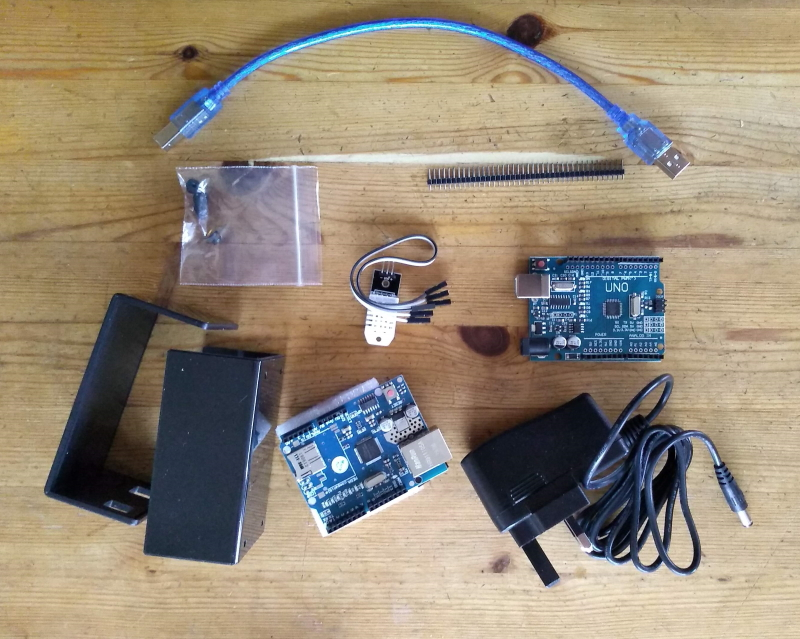
\includegraphics[width=0.8\textwidth]{components.jpg}
  \caption{Components}
\end{figure}


\begin{tabular}{ll}
  \textbf{Component} & \textbf{Cost} \\ 
  \hline
  Arduino Uno Rev3, ATmega328P, CH340G Compatible Board & \pounds 5.79 \\
  UK 9V AC/DC Power Supply Adapter Plug for Arduino Uno & \pounds 7.95 \\
  Ethernet Shield LAN W5100 for Arduino Uno & \pounds 7.75 \\
  DHT22 AM2302 Digital Temperature and Humidity Sensor & \pounds 6.90 \\
  0.25 Watt Metal Film Resistor 10K Ohm & \pounds 0.99 \\
  Uno Ethernet Shield Case & \pounds 10.36 \\
  \hline
  Total cost in November 2020 & \textbf{\pounds 39.74}  \\
\end{tabular}

\subsection{Sensor}

AM2302 capacitive humidity sensing digital temperature and humidity module is one that contains the
compound has been calibrated digital signal output of the temperature and humidity sensors. 



\subsection{Sensor}

%%%%%%%%%%%%%%%%%%%%%%%%%%%%%%%%%%%%%%%%%%%%%%%%%%%%%%%%%%%%
\section{Wiring}

Pull up resistor.



\begin{figure}[H]
  \centering
  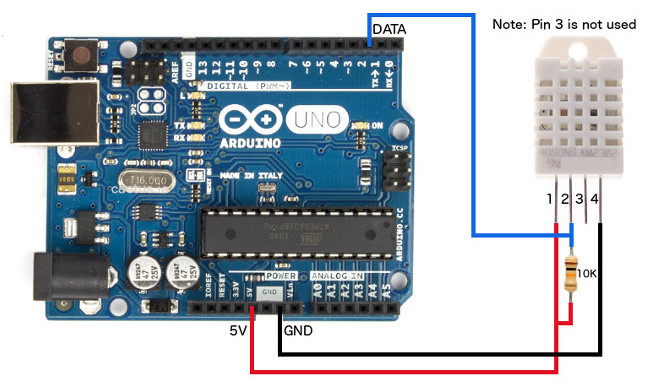
\includegraphics[width=0.8\textwidth]{wiring-dht22.jpg}
  \caption{Wiring diagram with pull up resistor}
\end{figure}


%%%%%%%%%%%%%%%%%%%%%%%%%%%%%%%%%%%%%%%%%%%%%%%%%%%%%%%%%%%%
\section{Programming}

Install 

\begin{itemize}
  \item VSCode \\
  \url{https://code.visualstudio.com/}
  \item Platformio \\
  \url{https://marketplace.visualstudio.com/items?itemName=platformio.platformio-ide}
\end{itemize}



Platform io

Include serial for output to monitor

\begin{flushleft} \small
\begin{minipage}{\linewidth}\label{scrap1}\raggedright\small
\NWtarget{nuweb4a}{}\verb@"../src/shit.cpp"@\nobreak\ {\footnotesize{4a}}$\equiv$
\vspace{-1ex}
\begin{list}{}{\setlength{\leftmargin}{1em}} \item
\mbox{}\verb@#include <Arduino.h>@\\
\mbox{}\verb@@$\langle\,${\itshape libraries}\ {\footnotesize \NWlink{nuweb4b}{4b}},\ ...\,$\rangle\,$\verb@@\\
\mbox{}\verb@@$\langle\,${\itshape configuration}\ {\footnotesize \NWlink{nuweb4c}{4c}},\ ...\,$\rangle\,$\verb@@\\
\mbox{}\verb@@$\langle\,${\itshape functions}\ {\footnotesize \NWlink{nuweb5b}{5b}}\,$\rangle\,$\verb@@\\
\mbox{}\verb@@\\
\mbox{}\verb@void setup() @\\
\mbox{}\verb@{@\\
\mbox{}\verb@  // Open serial communications and wait for the port to open.@\\
\mbox{}\verb@  Serial.begin(9600);@\\
\mbox{}\verb@  while (!Serial) @\\
\mbox{}\verb@  {@\\
\mbox{}\verb@    ; // Wait for serial port to connect (only needed for native USB ports).@\\
\mbox{}\verb@  }@\\
\mbox{}\verb@  @$\langle\,${\itshape setup}\ {\footnotesize \NWlink{nuweb5a}{5a}}\,$\rangle\,$\verb@@\\
\mbox{}\verb@}@\\
\mbox{}\verb@@\\
\mbox{}\verb@void loop() @\\
\mbox{}\verb@{@\\
\mbox{}\verb@  @$\langle\,${\itshape loop}\ {\footnotesize \NWlink{nuweb??}{??}}\,$\rangle\,$\verb@@\\
\mbox{}\verb@}@\\
\mbox{}{\NWsep}
\end{list}
\vspace{-1ex}
\end{minipage}
\end{flushleft}

%%%%%%%%%%%%%%%%%%%%%%%%%%%%%%%%%%%%%%%%%%%%%%%%%%%%%%%%%%%%
\subsection{Sensor}

Why Adafruit library?

Why DHT library?

Serial Peripheral Interface (SPI) is a synchronous serial data protocol
used by microcontrollers for communicating with peripheral devices quickly over short distances.

\begin{flushleft} \small
\begin{minipage}{\linewidth}\label{scrap2}\raggedright\small
\NWtarget{nuweb4b}{}$\langle\,${\itshape libraries}\nobreak\ {\footnotesize{4b}}$\,\rangle\equiv$
\vspace{-1ex}
\begin{list}{}{\setlength{\leftmargin}{1em}} \item
\mbox{}\verb@// Sensor libraries:@\\
\mbox{}\verb@#include <Adafruit_Sensor.h>@\\
\mbox{}\verb@#include <DHT.h>@\\
\mbox{}\verb@#include <SPI.h>@\\
\mbox{}{\NWsep}
\end{list}
\vspace{-1ex}
\vspace{-1ex}
\footnotesize
\begin{list}{}{\setlength{\itemsep}{-\parsep}\setlength{\itemindent}{-\leftmargin}}
\item \NWtxtMacroDefBy\ \NWlink{nuweb4b}{4b}, \NWlink{nuweb5c}{5c}.
\item \NWtxtMacroRefIn\ \NWlink{nuweb4a}{4a}.
\end{list}
\end{minipage}
\end{flushleft}

Pin and DHT type
DHT11 cheaper and less precise probably would be just as good for our situation
DHT21 (AM2301)

Register the pin used see wiring.

\begin{flushleft} \small
\begin{minipage}{\linewidth}\label{scrap3}\raggedright\small
\NWtarget{nuweb4c}{}$\langle\,${\itshape configuration}\nobreak\ {\footnotesize{4c}}$\,\rangle\equiv$
\vspace{-1ex}
\begin{list}{}{\setlength{\leftmargin}{1em}} \item
\mbox{}\verb@#define DHTPIN 2@\\
\mbox{}\verb@#define DHTTYPE DHT22   // DHT 22  (AM2302)@\\
\mbox{}\verb@// Initialize DHT sensor for normal 16mhz Arduino:@\\
\mbox{}\verb@DHT dht = DHT(DHTPIN, DHTTYPE);@\\
\mbox{}\verb@// globals to store readings@\\
\mbox{}\verb@float temperature = 0;@\\
\mbox{}\verb@float humidity = 0;@\\
\mbox{}{\NWsep}
\end{list}
\vspace{-1ex}
\vspace{-1ex}
\footnotesize
\begin{list}{}{\setlength{\itemsep}{-\parsep}\setlength{\itemindent}{-\leftmargin}}
\item \NWtxtMacroDefBy\ \NWlink{nuweb4c}{4c}, \NWlink{nuweb5d}{5d}.
\item \NWtxtMacroRefIn\ \NWlink{nuweb4a}{4a}.
\end{list}
\end{minipage}
\end{flushleft}

The sensor needs to begin, why?

\begin{flushleft} \small
\begin{minipage}{\linewidth}\label{scrap4}\raggedright\small
\NWtarget{nuweb5a}{}$\langle\,${\itshape setup}\nobreak\ {\footnotesize{5a}}$\,\rangle\equiv$
\vspace{-1ex}
\begin{list}{}{\setlength{\leftmargin}{1em}} \item
\mbox{}\verb@  Serial.println("Set up sensor");@\\
\mbox{}\verb@  dht.begin();@\\
\mbox{}{\NWsep}
\end{list}
\vspace{-1ex}
\vspace{-1ex}
\footnotesize
\begin{list}{}{\setlength{\itemsep}{-\parsep}\setlength{\itemindent}{-\leftmargin}}
\item \NWtxtMacroRefIn\ \NWlink{nuweb4a}{4a}.
\end{list}
\end{minipage}
\end{flushleft}

Set the values in the globals,
could have passed stuff around.

\begin{flushleft} \small
\begin{minipage}{\linewidth}\label{scrap5}\raggedright\small
\NWtarget{nuweb5b}{}$\langle\,${\itshape functions}\nobreak\ {\footnotesize{5b}}$\,\rangle\equiv$
\vspace{-1ex}
\begin{list}{}{\setlength{\leftmargin}{1em}} \item
\mbox{}\verb@void readSensor()@\\
\mbox{}\verb@{@\\
\mbox{}\verb@  // Read the humidity in %:@\\
\mbox{}\verb@  humidity = dht.readHumidity();@\\
\mbox{}\verb@  // Read the temperature as Celsius:@\\
\mbox{}\verb@  temperature = dht.readTemperature();@\\
\mbox{}\verb@  // Check if any reads failed and exit early (to try again):@\\
\mbox{}\verb@  if (isnan(humidity) || isnan(temperature)) @\\
\mbox{}\verb@  {@\\
\mbox{}\verb@    Serial.println("Failed to read from sensor");@\\
\mbox{}\verb@    return;@\\
\mbox{}\verb@  }@\\
\mbox{}\verb@}@\\
\mbox{}{\NWsep}
\end{list}
\vspace{-1ex}
\vspace{-1ex}
\footnotesize
\begin{list}{}{\setlength{\itemsep}{-\parsep}\setlength{\itemindent}{-\leftmargin}}
\item \NWtxtMacroRefIn\ \NWlink{nuweb4a}{4a}.
\end{list}
\end{minipage}
\end{flushleft}


%%%%%%%%%%%%%%%%%%%%%%%%%%%%%%%%%%%%%%%%%%%%%%%%%%%%%%%%%%%%
\subsection{Ethernet Client}

aWOT is in version 3

\verb|lasselukkari/aWOT@0.0.0-alpha+sha.bf07e6371c|


\begin{flushleft} \small
\begin{minipage}{\linewidth}\label{scrap6}\raggedright\small
\NWtarget{nuweb5c}{}$\langle\,${\itshape libraries}\nobreak\ {\footnotesize{5c}}$\,\rangle\equiv$
\vspace{-1ex}
\begin{list}{}{\setlength{\leftmargin}{1em}} \item
\mbox{}\verb@// Ethernet shield@\\
\mbox{}\verb@#include <Ethernet.h>@\\
\mbox{}\verb@#include <aWOT.h>@\\
\mbox{}{\NWsep}
\end{list}
\vspace{-1ex}
\vspace{-1ex}
\footnotesize
\begin{list}{}{\setlength{\itemsep}{-\parsep}\setlength{\itemindent}{-\leftmargin}}
\item \NWtxtMacroDefBy\ \NWlink{nuweb4b}{4b}, \NWlink{nuweb5c}{5c}.
\item \NWtxtMacroRefIn\ \NWlink{nuweb4a}{4a}.
\end{list}
\end{minipage}
\end{flushleft}


\begin{flushleft} \small
\begin{minipage}{\linewidth}\label{scrap7}\raggedright\small
\NWtarget{nuweb5d}{}$\langle\,${\itshape configuration}\nobreak\ {\footnotesize{5d}}$\,\rangle\equiv$
\vspace{-1ex}
\begin{list}{}{\setlength{\leftmargin}{1em}} \item
\mbox{}\verb@// Enter a MAC address and IP address for your controller below.@\\
\mbox{}\verb@// The IP address will be dependent on your local network:@\\
\mbox{}\verb@byte mac[] = {@\\
\mbox{}\verb@  0xDE, 0xAD, 0xBE, 0xEF, 0xFE, 0xED@\\
\mbox{}\verb@};@\\
\mbox{}\verb@IPAddress ip(10, 0, 21, 211);@\\
\mbox{}\verb@// Initialize the Ethernet server library@\\
\mbox{}\verb@// with the IP address and port you want to use@\\
\mbox{}\verb@// (port 80 is default for HTTP):@\\
\mbox{}\verb@EthernetServer server(80);@\\
\mbox{}\verb@Application app;@\\
\mbox{}{\NWsep}
\end{list}
\vspace{-1ex}
\vspace{-1ex}
\footnotesize
\begin{list}{}{\setlength{\itemsep}{-\parsep}\setlength{\itemindent}{-\leftmargin}}
\item \NWtxtMacroDefBy\ \NWlink{nuweb4c}{4c}, \NWlink{nuweb5d}{5d}.
\item \NWtxtMacroRefIn\ \NWlink{nuweb4a}{4a}.
\end{list}
\end{minipage}
\end{flushleft}


\begin{flushleft} \small
\begin{minipage}{\linewidth}\label{scrap8}\raggedright\small
\NWtarget{nuweb??}{}$\langle\,${\itshape loop}\nobreak\ {\footnotesize{??}}$\,\rangle\equiv$
\vspace{-1ex}
\begin{list}{}{\setlength{\leftmargin}{1em}} \item
\mbox{}\verb@  // Wait a couple of seconds between measurements.@\\
\mbox{}\verb@  delay(2000);@\\
\mbox{}\verb@  // Reading temperature or humidity takes about 250 milliseconds@\\
\mbox{}\verb@  // Sensor readings may also be up to 2 seconds 'old'@\\
\mbox{}\verb@  readSensor();@\\
\mbox{}\verb@  serialPrintReadings();@\\
\mbox{}\verb@  EthernetClient client = server.available();@\\
\mbox{}\verb@  if (client.connected()) {@\\
\mbox{}\verb@    app.process(&client);@\\
\mbox{}\verb@    client.stop();@\\
\mbox{}\verb@  }@\\
\mbox{}{\NWsep}
\end{list}
\vspace{-1ex}
\vspace{-1ex}
\footnotesize
\begin{list}{}{\setlength{\itemsep}{-\parsep}\setlength{\itemindent}{-\leftmargin}}
\item \NWtxtMacroRefIn\ \NWlink{nuweb4a}{4a}.
\end{list}
\end{minipage}
\end{flushleft}

%%%%%%%%%%%%%%%%%%%%%%%%%%%%%%%%%%%%%%%%%%%%%%%%%%%%%%%%%%%%
\subsection{Upload}

Drivers on PC.



%%%%%%%%%%%%%%%%%%%%%%%%%%%%%%%%%%%%%%%%%%%%%%%%%%%%%%%%%%%%
\subsection{Testing}

\begin{verbatim}
  --- Quit: Ctrl+C | Menu: Ctrl+T | Help: Ctrl+T followed by Ctrl+H ---
  Webserver set up
  Sensor set up
  Humidity: 55.90 % | Temperature: 22.10 C
  Humidity: 56.30 % | Temperature: 22.20 C
\end{verbatim}


Rather than link up to a router

\begin{itemize}
  \item Assign a manual IP address to the laptop's ethernet connection say 10.0.21.1.
  \item Subnet mask 255.255.255.0.
  \item Assign a manual IP address to the Arduino's ethernet, say 10.0.21.211.
  \item Subnet mask 255.255.255.0.
  \item Leave the default Gateway empty.
  \item Use an ethernet patch cable to link the two (since 100BaseT onwards it doesn't have to be a special cross over cable).
  \item You should then be able to get your Arduino site up on \url{http://192.168.0.2} from the laptop.
\end{itemize}
  
This is the endpoint at \url{http://10.0.21.211/metrics}.
  
\begin{verbatim}
  > curl 10.0.21.211
  # HELP temperature is the last temperature reading in degrees celsius
  # TYPE temp gauge
  temperature 23.30
  # HELP humidity is the last relative humidity reading as a percentage
  # TYPE humidity gauge
  humidity 47.60
\end{verbatim}

\verb|docker-compose up|

\begin{figure}[H]
  \centering
  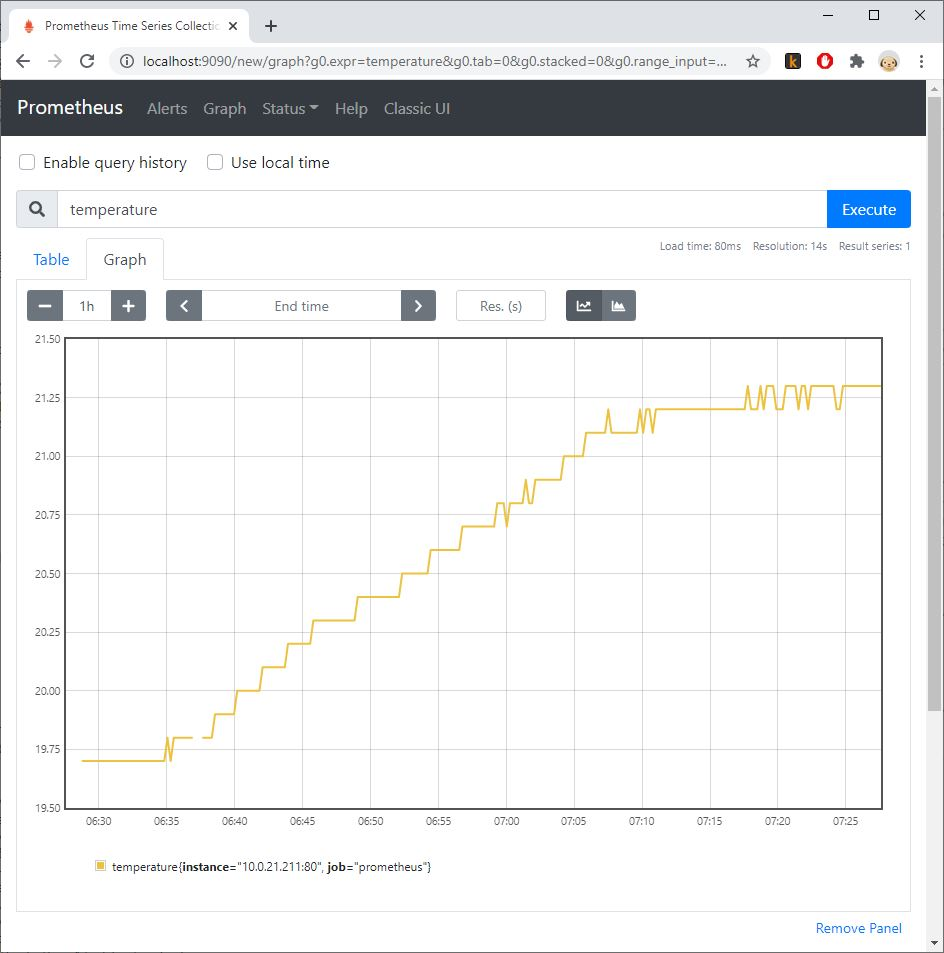
\includegraphics[width=0.8\textwidth]{graph.jpg}
  \caption{Temperature graph}
\end{figure}
  

%%%%%%%%%%%%%%%%%%%%%%%%%%%%%%%%%%%%%%%%%%%%%%%%%%%%%%%%%%%%
\section{Packaging}

\begin{figure}[H]
  \centering
  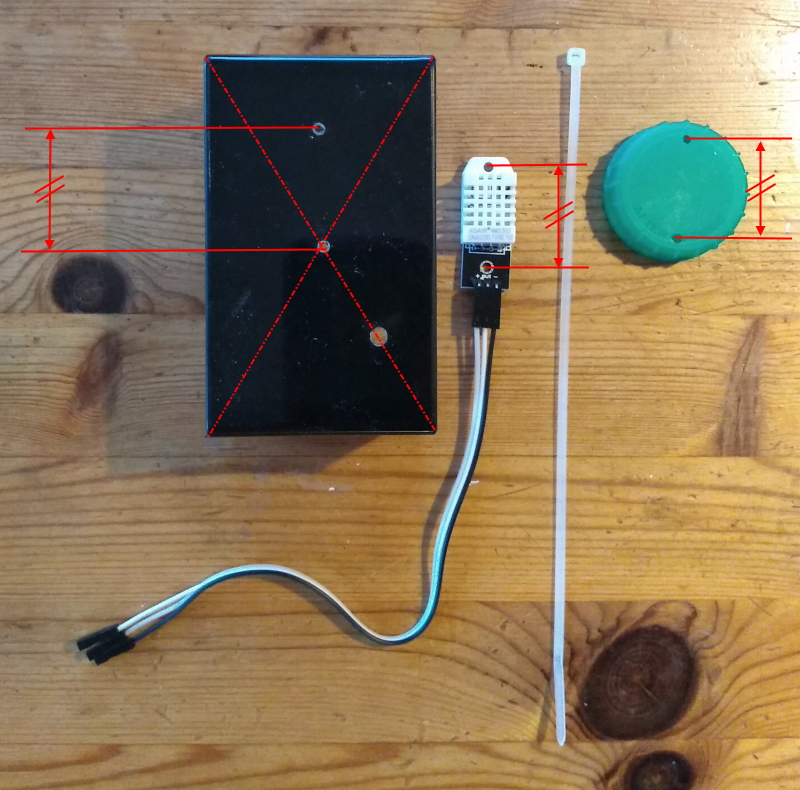
\includegraphics[width=0.8\textwidth]{sensor-mount.jpg}
  \caption{Components for mounting the sensor}
\end{figure}

2.5 mm holes and 4 mm holes.

\begin{figure}[H]
  \centering
  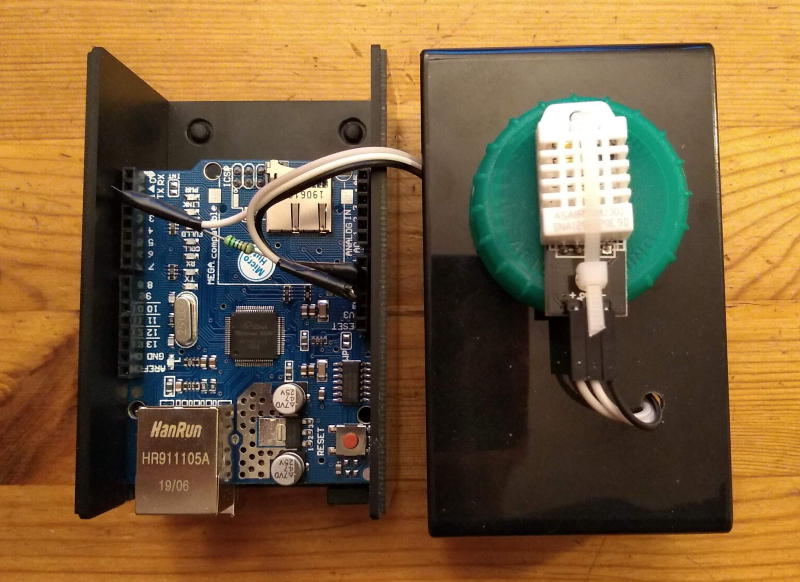
\includegraphics[width=0.8\textwidth]{packaging.jpg}
  \caption{Mounted sensor and wiring}
\end{figure}

\end{document}